\documentclass{beamer}
\usepackage{amsmath}
\usepackage{listings}
\usepackage{amssymb}
\usepackage{xeCJK}
\usepackage{amsmath}

\begin{document}
    \begin{frame}
    \title{How to synchronize automata $\mathcal{A}$ and $\mathcal{B}_{\neg\phi}$}
    \author{林奇峰\\ Qifeng Lin \\ 17214656}
    \maketitle
    \end{frame}

    \begin{frame}
        \frametitle{recall synchronization of automata}
        cartesian product of automata $\mathcal{A}_1,\mathcal{A}_2,\dots$ \\
            \begin{itemize}
                \item $Q=Q_1$x...x$Q_n$;
                \item $E=\prod_{}{}_{1\leq i \leq n}(E_i\cup\{-\})$;
                \item $T=\left.\{ ((q_1,...,q_n),(e_1,\dots,e_n)(q_1',...,q_n')) |  for\right.$ $all$ $i$, $e_i='-'$ and $q_i'=q_i$, or $e_i\neq '-'$ and $(q_i,e_i,q_i')\in T_i \left.\right\} $;
                \item $q_0=(q_{0,1},...,q_{0,n})$;
                \item $l((q_1,...,q_n))=\cup _{1\leq i \leq n}l_i(q_i)$
            \end{itemize}

        synchronization set \\
            \quad $   Sync \subseteq \prod_{1\leq i \leq n}^{}(E_i\cup\{-\})$
    \end{frame}

    \begin{frame}
        \frametitle{task: synchronize two automata}
        automaton $\mathcal{A}$\\
        \begin{figure}
            \centering
            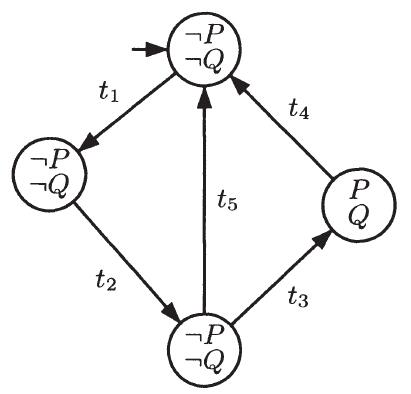
\includegraphics[width=2.0in,height=2.0in]{3_2.jpg}
        \end{figure}
        automaton $\mathcal{B}_{\neg\phi}$
        \begin{figure}
            \centering
            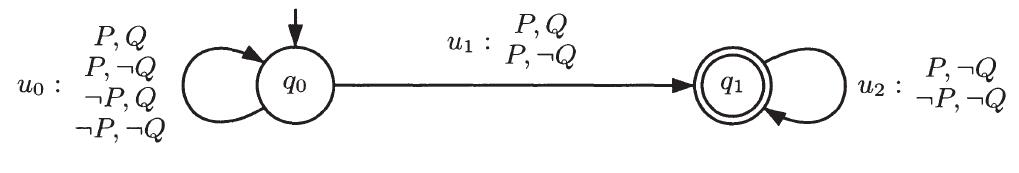
\includegraphics[width=4.0in]{3_1.jpg}
        \end{figure}
    \end{frame}
    \begin{frame}
        \frametitle{construct cartesian product}
        \begin{itemize}
          \item $Q_1$=\{$(\neg P$,$\neg Q)_1$,$(\neg P, \neg Q)_2$,($\neg P, \neg Q)_3$,$(P,Q)$\}\\
                $Q_2$=\{$q_0$,$q_1$\}
          \item $E=\{(t_1,u_0),(t_2,u_0),(t_3,u_0),(t_4,u_0),(t_5,u_0),$\\
                \qquad $(t_1,u_1),(t_2,u_1),(t_3,u_1),(t_4,u_1),(t_5,u_1),$\\
                \qquad $(t_1,u_3),(t_2,u_3),(t_3,u_3),(t_4,u_3),(t_5,u_3)\}$
          \item $T=$\{($(\neg P, \neg Q)_1$, $q_0$),$(t_1,u_0)$,($(\neg P, \neg Q)_2$, $q_0$)),\\
                \qquad($(\neg P, \neg Q)_2$, $q_0$),$(t_2,u_0)$,($(\neg P, \neg Q)_3$, $q_0$),\\
                \qquad\dots\}
          \item initial state $q=((\neg P$,$\neg Q)_1,q_0)$
          \item
                  $l= \{((\neg P,\neg Q)_1,q_0)\mapsto(\neg P,\neg Q),$\\
                  \qquad$ ((P,Q),q_0)\mapsto (P,Q) $\\
                 \qquad$   \dots \}$
        \end{itemize}


    \end{frame}

    \begin{frame}
        \begin{figure}
            \centering
            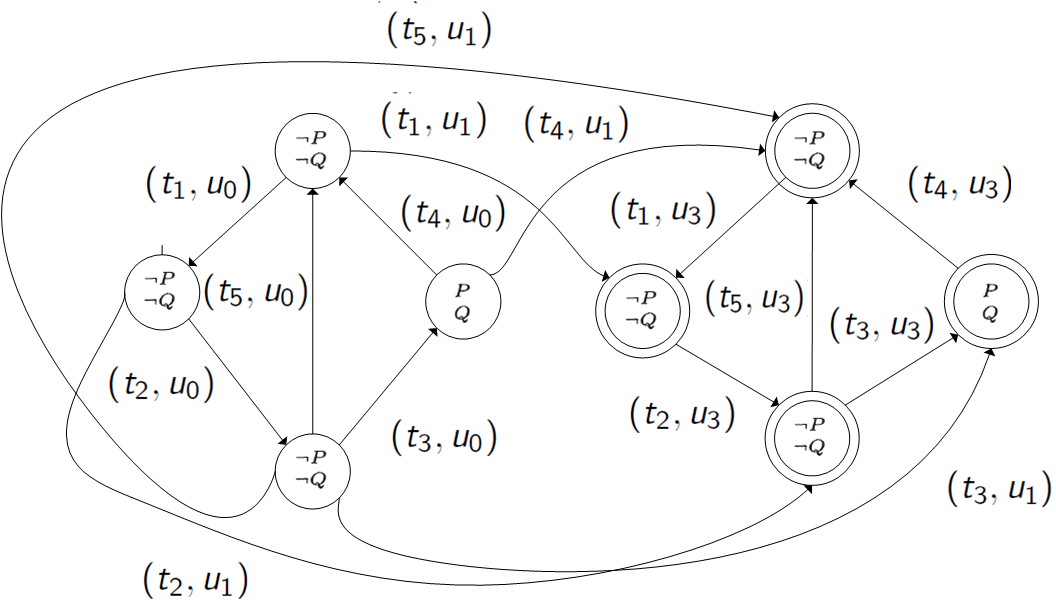
\includegraphics[width=4.0in]{cartesian.png}
        \end{figure}
    \end{frame}

    \begin{frame}
        \frametitle{synchronization rule}
        $(t,u)$ is possible only if $t$ leaves a state that satisfies $u$, denote as $t\otimes u$ \\
        for example \\
        \begin{itemize}
          \item $t\otimes u_1$ happens when t leaves a state satisfying P\\
          \item $u_1$=$\{(P,Q),(P,\neg Q)\}$ \\
                therefore, in set \{$(t_1,u_1),(t_2,u_1),(t_3,u_1),(t_4,u_1),(t_5,u_1)$\}\\
          \item only $t_4\otimes u_1$ is possible
        \end{itemize}

        synchronization set:\
        $Sync=\{(t_1,u_0),(t_2,u_0),(t_3,u_0),(t_4,u_0),(t_5,u_0),$\\
        \quad\qquad$(t_4,u_1),$\\
        \quad\qquad $(t_1,u_3),(t_2,u_3),(t_3,u_3),(t_5,u_3)\}$
    \end{frame}

    \begin{frame}
        \frametitle{automaton $\mathcal{A}\otimes\mathcal{B}_{\neg\phi}$}
        \begin{figure}
            \centering
            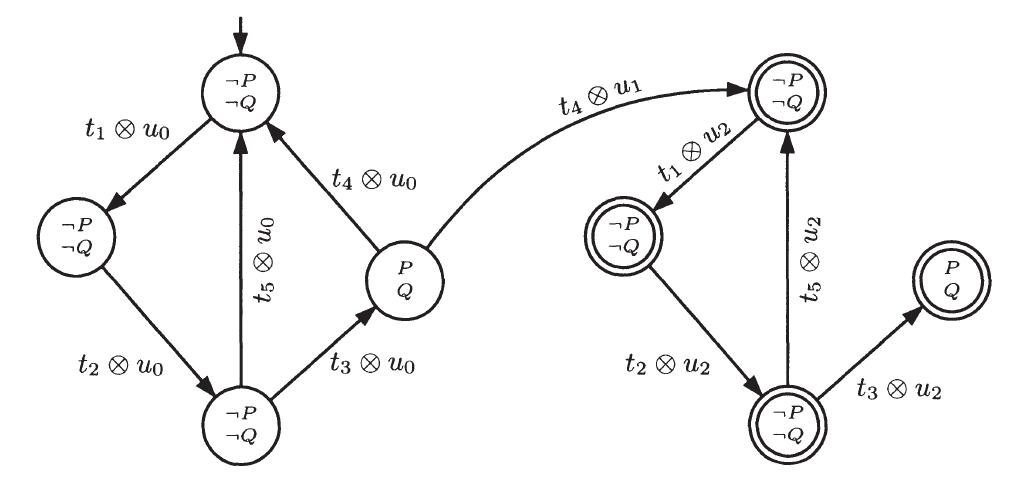
\includegraphics[width=4.0in]{3_3.jpg}
        \end{figure}

    \end{frame}

    \begin{frame}
    \end{frame}
\end{document} 